% XeLaTeX can use any Mac OS X font. See the setromanfont command below.
% Input to XeLaTeX is full Unicode, so Unicode characters can be typed directly into the source.

% The next lines tell TeXShop to typeset with xelatex, and to open and save the source with Unicode encoding.

%!TEX TS-program = xelatex
%!TEX encoding = UTF-8 Unicode

\documentclass[12pt]{article}
\usepackage{geometry}                % See geometry.pdf to learn the layout options. There are lots.
\geometry{letterpaper}                   % ... or a4paper or a5paper or ... 

\geometry{left=1in}
\geometry{right=1in}
\geometry{bottom=1.9in}
\geometry{top=1in}

%
%Setting the font
%
\usepackage{times}

%
%Rotating tables (e.g. sideways when too long)
%
\usepackage{rotating}

%
%For multiple rows in tables
%
\usepackage{multirow}

% 
%Line numbering in verse environment
%
\usepackage{lineno} 

%
%Fancy-header package to modify header/page numbering (insert last name)
%
\usepackage{fancyhdr}
\pagestyle{fancy}
\lhead{} 
\chead{} 
\rhead{Quan \thepage} 
\lfoot{} 
\cfoot{} 
\rfoot{} 
\renewcommand{\headrulewidth}{0pt} 
\renewcommand{\footrulewidth}{0pt} 
%To make sure we actually have header 0.5in away from top edge
%12pt is one-sixth of an inch. Subtract this from 0.5in to get headsep value
\setlength{\headsep}{1in}

\usepackage{setspace}
\doublespacing

\usepackage{booktabs}
\usepackage[american]{babel}
\usepackage{csquotes}
\usepackage[backend=bibtex,style=mla]{biblatex}
\usepackage{url}
\usepackage[parfill]{parskip}
\usepackage{listings}
 \usepackage{float}

\usepackage{titlesec}
\usepackage{amsmath}
\usepackage{amssymb}

\usepackage{xcolor}

\lstset{language=python}
\lstset{breaklines}
\definecolor{mygreen}{rgb}{0,0.6,0}
\definecolor{mygray}{rgb}{0.5,0.5,0.5}
\definecolor{mymauve}{rgb}{0.58,0,0.82}

\lstset{numbers=left, 
numberstyle=\tiny, 
keywordstyle=\color{blue},
commentstyle=\color{mygreen},    % comment style
rulecolor=\color{black},
frame=shadowbox, 
rulesepcolor=\color{red!20!green!20!blue!20},
stringstyle=\color{mymauve},     % string literal style
title=\lstname,
showspaces=false,
showstringspaces=false
}

\title{}
\author{}
\date{}                                           % Activate to display a given date or no date

\addbibresource{bib.bib}
\begin{document}

\begin{flushleft}
%%%%First page name, class, etc
Shengjie Quan\\
Professor: Adam C. Champion\\
CSE 3461	 \\
\today \\
\end{flushleft}

%%%%Title
\begin{center}
Response to Homework 4
\end{center}

%%%%Changes paragraph indentation to 0.5in
\setlength{\parindent}{0.5in}

\begin{singlespace}

\begin{enumerate}

\item Below is the drawing of links over which packets will be forwarded using RPF:
	\begin{figure}[h]
	\centering
	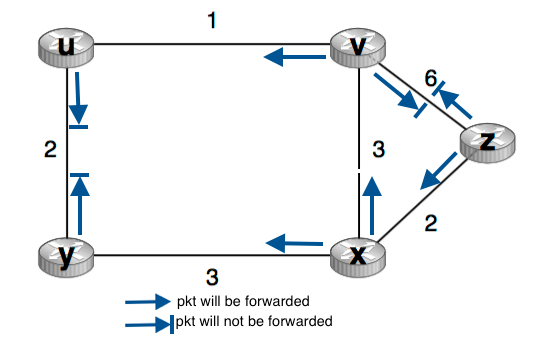
\includegraphics[width=0.64\textwidth]{1a} 
	\end{figure}

\item Consider the topology below:
	\begin{figure}[h]
	\centering
	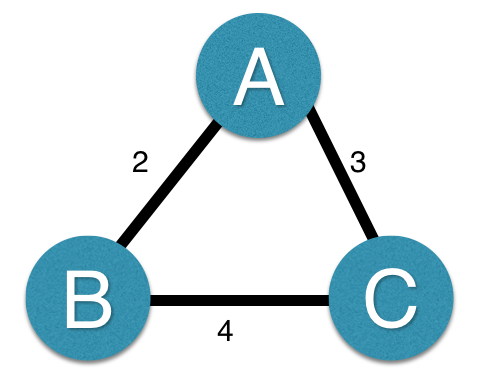
\includegraphics[width=0.4\textwidth]{2a} 
	\end{figure}\\
	The minimal spanning tree is as follow:
	\begin{figure}[h]
	\centering
	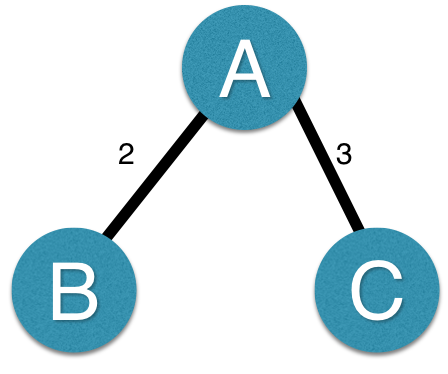
\includegraphics[width=0.4\textwidth]{2b} 
	\end{figure}\\
	However, the least-unicast-cost path tree when node C is designated to be the source is as follow:
	\begin{figure}[h]
	\centering
	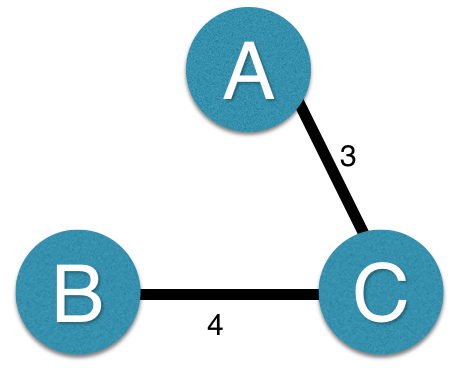
\includegraphics[width=0.4\textwidth]{2c} 
	\end{figure}
\item Below is the matrix with even parity bits added:
	\begin{table}[h]
	\centering
	\begin{tabular}{|l|l|l|l|l|l|}
	\hline
	Data       &   &   &   &   & Parity Bit \\ \hline
	           & 1 & 1 & 1 & 0 & 1          \\ \hline
	           & 0 & 1 & 1 & 0 & 0          \\ \hline
	           & 1 & 0 & 0 & 1 & 0          \\ \hline
	           & 1 & 1 & 0 & 1 & 1          \\ \hline
	Parity Bit & 1 & 1 & 0 & 0 & 0          \\ \hline
	\end{tabular}
	\end{table}
\item Since Ethernet use CSMA/CD to resolve collision so its efficiency can be calculated by using the CSMA/CD efficiency formula, Efficiency$\; = \frac{1}{1 + 5\,d_{prop} \div \,d_{trans}}$.\\
For $d_{prop}$, the maximum time it takes signal energy to propagate between any two adapters, it can be calculated by $d_{prop} = \frac{L}{c}$ where $L$ is the length of the wire and $c=2\times10^8 \, m/s$ is the signal propagation speed. \\
For $d_{trans}$, the time to transmit a maximum-size frame, it can be calculated by $d_{trans} = \frac{64 \times 8}{100\times1000^2}$ where $64 \times 8$ is the size of a frame in bit and $100\times1000^2$ is the speed of transmission (assume 1 Mbps = 1000 kbps and 1 kbps = 1000 bps). 
So we have a equation, $0.7 = \frac{1}{1 + 5\,\frac{L}{c} \div \, \frac{64 \times 8}{100\times1000^2}}$, and solving for $L$ we get $L = 87.771 m$.\\
So to achieve efficiency of 0.7 the maximum distance should be 87.771 m.
\item
\begin{itemize}
	\item[(a.)]
	The efficiency can be treated as a function of probability , $p$. So we have $E(p) = N\,p(1-p)^{N-1}$. We than take its first order derivative. So we have $E'(p) = \frac{-(p\,N-1)(1-p)^N\,N}{(p-1)^2}$. Let $E'(p) = 0$, we solving for $p$ get $p=\frac{1}{N}$. So when $p=\frac{1}{N}$, the function is at maximum.
	\item[(b.)]
	Let's denote the $p$ find in (a.) as $p^* = \frac{1}{N}$. So $E(p^*) = \frac{N \, (\frac{N-1}{N})^N}{N-1}$. Using calculator to calculate the limit $\lim_{N \to \infty} \frac{N \, (\frac{N-1}{N})^N}{N-1} = \frac{1}{e}$.
\end{itemize}

\item
	Below is the print out of the command /sbin/ifconfig -a :
	\begin{lstlisting}[basicstyle=\ttfamily\scriptsize]
% /sbin/ifconfig -a
eth0      Link encap:Ethernet  HWaddr 00:13:72:54:CC:73  
          inet addr:164.107.113.20  Bcast:164.107.113.255  Mask:255.255.255.0
          UP BROADCAST RUNNING MULTICAST  MTU:1500  Metric:1
          RX packets:1588805570 errors:10 dropped:0 overruns:0 frame:5
          TX packets:2458269358 errors:0 dropped:0 overruns:0 carrier:0
          collisions:0 txqueuelen:1000 
          RX bytes:552010372854 (514.0 GiB)  TX bytes:2059466014216 (1.8 TiB)

eth1      Link encap:Ethernet  HWaddr 00:13:72:54:CC:74  
          BROADCAST MULTICAST  MTU:1500  Metric:1
          RX packets:0 errors:0 dropped:0 overruns:0 frame:0
          TX packets:0 errors:0 dropped:0 overruns:0 carrier:0
          collisions:0 txqueuelen:1000 
          RX bytes:0 (0.0 b)  TX bytes:0 (0.0 b)

lo        Link encap:Local Loopback  
          inet addr:127.0.0.1  Mask:255.0.0.0
          inet6 addr: ::1/128 Scope:Host
          UP LOOPBACK RUNNING  MTU:65536  Metric:1
          RX packets:321616353 errors:0 dropped:0 overruns:0 frame:0
          TX packets:321616353 errors:0 dropped:0 overruns:0 carrier:0
          collisions:0 txqueuelen:0 
          RX bytes:165346718548 (153.9 GiB)  TX bytes:165346718548 (153.9 GiB)
	\end{lstlisting}
The command, ifconfig, is used to show the network interface configuration. From the print out, we can see that there are three interface on a stdlinux machine. The interface, eth0 is the actually network card with MAC address of 00:13:72:54:CC:73. It is assigned the IP address of 164.107.113.20. MTU is its max transmission unit and for eth0, its MTU is set to 1500.\\
eth1 is another interface with unknown purpose.\\
The interface, lo, a virtual network interface which refers to the machine itself.\\\\

Below is a print out of command /sbin/arp -a :
	\begin{lstlisting}[basicstyle=\ttfamily\scriptsize]
% /sbin/arp -a
beta.cse.ohio-state.edu (164.107.113.18) at 00:13:72:54:cc:4f [ether] on eth0
sl3.cse.ohio-state.edu (164.107.113.12) at 00:50:56:95:55:53 [ether] on eth0
hsrp113.cse.ohio-state.edu (164.107.113.1) at 00:23:9c:46:f2:01 [ether] on eth0
	\end{lstlisting}
The second command arp is the abbreviation of Address Resolution Protocol. Its function showing the result of Address Resolution Protocol is pretty self-evident.\\
From the print out we can see that \textbf{beta.cse.ohio-state.edu (164.107.113.18)} is resolved to \textbf{00:13:72:54:cc:4f}. We can also see that \textbf{sl3.cse.ohio-state.edu (164.107.113.12)} is resolved to \textbf{00:50:56:95:55:53} and \textbf{hsrp113.cse.ohio-state.edu (164.107.113.1)} is resolved to \textbf{00:23:9c:46:f2:01}.
\end{enumerate}
\end{singlespace}

\clearpage

\printbibliography
\end{document}  